\documentclass[tikz,border=10pt]{standalone}
\usepackage{tikz}
\usetikzlibrary{arrows.meta,positioning,calc}

\tikzset{
  block/.style={
    draw,
    rectangle,
    minimum width=2.5cm,
    minimum height=1.0cm,
    align=center,
    line width=1.1pt,
    fill=white
  },
  sum/.style={
    draw,
    circle,
    minimum size=7mm,
    inner sep=0pt,
    line width=1.1pt,
    fill=white
  },
  tap/.style={
    circle,
    minimum size=1.8mm,
    inner sep=0pt,
    draw=black,
    fill=black
  },
  signal/.style={-{Latex[length=3mm,width=2mm]}, line width=1.1pt},
  flowlabel/.style={font=\small, fill=white, inner sep=1pt},
  nodetext/.style={font=\small},
  signmark/.style={font=\small}
}

\begin{document}
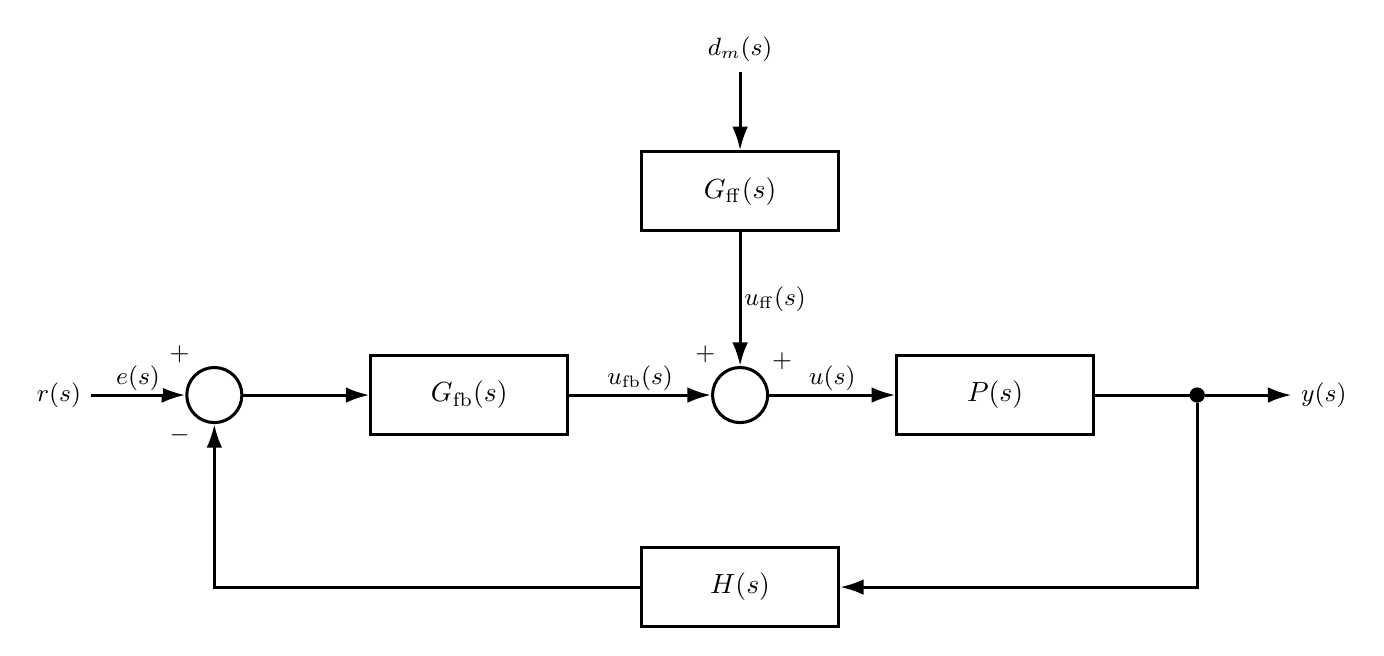
\begin{tikzpicture}[node distance=1.4cm and 1.2cm]
  \node[nodetext] (r) {$r(s)$};
  \node[sum, right=1.2cm of r] (sum1) {};
  \node[block, right=1.6cm of sum1] (cfb) {$G_{\mathrm{fb}}(s)$};
  \node[sum, right=1.8cm of cfb] (sum2) {};
  \node[block, right=1.6cm of sum2] (plant) {$P(s)$};
  \node[tap, right=1.2cm of plant] (ytap) {};
  \node[nodetext, right=1.1cm of ytap] (y) {$y(s)$};

  \node[block, above=1.7cm of sum2] (gff) {$G_{\mathrm{ff}}(s)$};
  \node[nodetext, above=1.0cm of gff] (dm) {$d_m(s)$};
  \node[block, below=1.55cm of sum2] (sensor) {$H(s)$};

  \draw[signal] (r) -- node[flowlabel, above] {$e(s)$} (sum1);
  \draw[signal] (sum1) -- (cfb);
  \draw[signal] (cfb) -- node[flowlabel, above] {$u_{\mathrm{fb}}(s)$} (sum2);
  \draw[signal] (sum2) -- node[flowlabel, above] {$u(s)$} (plant);
  \draw[signal] (plant) -- (ytap) -- (y);

  \draw[signal] (dm) -- (gff);
  \draw[signal] (gff) -- node[flowlabel, right] {$u_{\mathrm{ff}}(s)$} (sum2.north);

  \draw[signal] (ytap) |- (sensor.east);
  \draw[signal] (sensor.west) -| (sum1.south);

  \node[signmark, above left=0.2mm and -0.7mm of sum1] {$+$};
  \node[signmark, below left=0.2mm and -0.7mm of sum1] {$-$};
  \node[signmark, above left=0.2mm and -0.7mm of sum2] {$+$};
  \node[signmark, above right=-0.7mm and 0.2mm of sum2] {$+$};
\end{tikzpicture}
\end{document}
